\documentclass[a4paper,12pt]{article}
\usepackage[utf8]{inputenc}
\usepackage[IL2]{fontenc}
\usepackage{listings}
\usepackage{amssymb}
\usepackage{amsmath}
\usepackage{url}
\usepackage{graphicx}
\usepackage[czech]{babel}
\title{Kolektivní investování}
\author{Marek Bryša, Jan Kovář}
\date{Brno, \today}
\begin{document}
\maketitle

\section{Úvod}

\section{Vybrané fondy v ČR}
	\subsection{AXA investiční společnost, a.s.}
		Francouzská skupina AXA je druhým největším správcem fondů v Evropě.\cite{axa_about} Její produkty mají v České republice nulové vstupní poplatky, ale klient hradí správní poplatky a výstupní v případě ukončení investice za kratší dobu než 5 let. Kompletní přehled poplatků je uveden v příloze \ref{axa}.
		
		Pro drobné investory jsou určeny všechny fondy se vstupní investicí 5~000 Kč. Výjimkou je AXA Corporate Fund, který má minimální vstupní investici 1~000~000 Kč a následnou 500~000 Kč.
		
		\subsubsection{AXA CZK Konto}
			AXA CZK Konto je otevřený podílový fond, který byl do 31.12.2011 klasifikován jako fond peněžního trhu, od 1.1.2012 se podle metodiky AKAT ČR jedná o smíšený fond.
			\begin{quote}
				Cílem investiční strategie je poskytnout podílníkům růst hodnoty jejich investice za podmínky, že celkový rizikový profil fondu minimalizuje možnost ztráty v horizontu 6 měsíců. Cíle je dosahováno investicemi do široce diverzifikovaného portfolia cenných papírů s fixním nebo variabilním úrokovým výnosem a aktivním řízením úrokového rizika.\footnote{\url{http://www.axa.cz/lide/podilove-fondy/czk-konto/popis}}
			\end{quote}
			
			Doporučeným investičním horizontem je minimálně 6 měsícu. Fond je vhodný pro investora s nízkou tolerancí k riziku, který neočekává vysoký výnos.
			
			Graf zhodnocení fondu je uveden v obrázku \ref{axa_czk_konto}. Fond připsal za 5 let 10.07\%, v průměru tedy 1.93\% ročně, přičemž za poslední rok 0.8\%. To je výrazně méně než nabízely a nabízejí spořící účty v bankách. Je vidět, že v době finanční krize mezi roky 2008 a 2009 byl fond velmi volatilní. 
			\begin{figure}[h!]
		  	\centering
				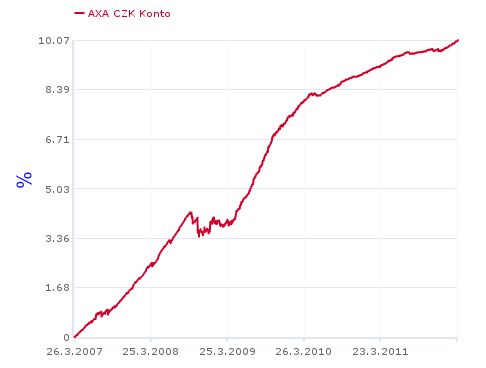
\includegraphics[width=0.6\textwidth]{axa_czk_konto.png}			
				\caption{Graf zhodnocení AXA CZK Konto za 5 let zdroj: http://www.axa.cz/fondy/porovnani/podilove.aspx?fund=29}
				\label{axa_czk_konto}
			\end{figure}
		\subsubsection{AXA CEE Dluhopisový fond}
			AXA CEE Dluhopisový fond je otevřený podílový fond klasifikovaný jako dluhopisový. 
			\begin{quote}
				Fond investuje do dluhopisů emitentů všech kategorií:
				\begin{itemize}
			    \item dluhopisů nadnárodních institucí
			    \item státních dluhopisů
			    \item bankovních dluhopisů
			    \item dluhopisů obchodních společností
			    \item komunálních dluhopisů emitovaných v krajinách střední a východní Evropy			
    	  \end{itemize}
    	  \footnote{\url{http://www.axa.cz/lide/podilove-fondy/cee-dluhopisovy/popis}}
		  \end{quote}						
			
			Doporučeným investičním horizontem jsou minimálně 3 roky. Fond je určen pro střednědobé investice s mírou rizika i výnosem o něco výššími než u fondu peněžního trhu.
			
			Graf zhodnocení fondu je uveden v obrázku \ref{axa_cee_dluh}. Výnos fondu je za 5 let 10.73\%, což je 2.05\% ročně. To je o málo více než fond CZK Konto, ale s mnohem vyšší volatilitou.
			
			\begin{figure}[h!]
		  	\centering
				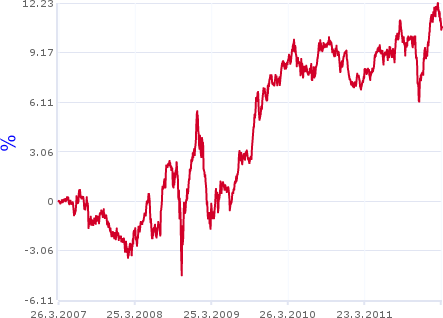
\includegraphics[width=0.6\textwidth]{axa_cee_dluh.png}			
				\caption{Graf zhodnocení AXA CEE Dluhopisový fond za 5 let zdroj: http://www.axa.cz/fondy/porovnani/podilove.aspx?fund=32}
				\label{axa_cee_dluh}
			\end{figure}
		\subsubsection{AXA CEE Akciový fond}
			AXA CEE Akciový fond je oficiálně klasifikován jako akciový fond.
			\begin{quote}
				Cílem fondu je dosahovat co nejvyššího dlouhodobého zhodnocení investic. Majetek fondu je tvořený především akciemi společností, které jsou lídry ve svém odvětví v regionu střední a východní Evropy. Největší podíl na portfoliu mají české, polské a maďarské společnosti. Odvětvová struktura portfolia není omezená, významně se na ní ale podílí energetický, telekomunikační a finanční sektor. Investice jsou směřované také do odvětví farmacie či strojírenství.\footnote{\url{http://www.axa.cz/lide/podilove-fondy/cee-akciovy/popis}}
			\end{quote}
			
			Doporučeným investičním horizontem je minimálně 5 let. Fond pro ivestora slibuje vyskoké zhodnocení v dlouhém obdobi, ale za cenu vysoké střednědobé volatility.
			
			Na grafu \ref{axa_cee_akc} dobře vidíme nebezpečí investic do akciových produktů ve středním období. Za 5 let fond ztratil 27.11\% hodnoty, v době finanční krize dokonce 52.3\%.			
			
			\begin{figure}[h!]
		  	\centering
				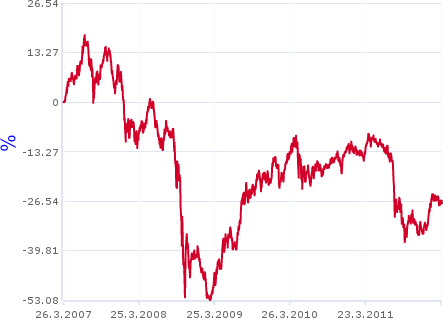
\includegraphics[width=0.6\textwidth]{axa_cee_akc.png}			
				\caption{Graf zhodnocení AXA CEE Akciový fond za 5 let zdroj: http://www.axa.cz/fondy/porovnani/podilove.aspx?fund=28}
				\label{axa_cee_akc}
			\end{figure}
	\subsection{Pioneer Asset Management, a.s. -- Rentier Invest}
		Společnost Pioneer působí na českém trhu od roku 1995. Přímo nabízí investice do fondů v CZK a přes svou lucemburskou matku také rodinu fondů v zahraničních měnách.\cite{pio_about} Pro osobní finance je zajímavým produktem program Rentier Invest.
		
		Program tvoří 7 na sebe navazujících linií s postupně se snižující rizikovostí a výnosem. První linie je určena pro 40-25 let před předpokládaným ukončením investice, druhá pro 25-15 let atd. Podrobný přehled je uveden na obrázku \ref{ri_linie}.
		
		Minimálně je možno investovat poprvé 30 000 Kč, následně 10 000 Kč nebo pravidelně 1 000 Kč. Vstupní polatky se s každou linií snižují, viz obrázek \ref{ri_cost}. Správcovské poplatky nejsou pro tento program na internetu k nalezení.
		\begin{figure}[h!]
		  	\centering
			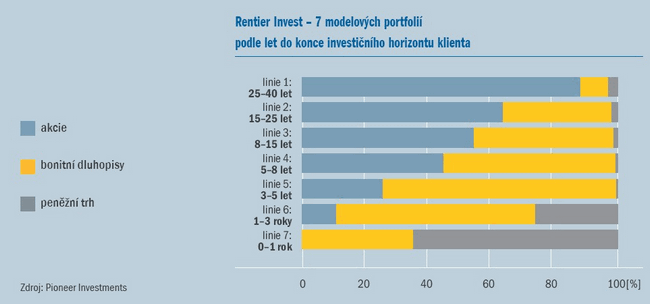
\includegraphics[width=0.8\textwidth]{graf_alokace_linii.png}			
			\caption{Graf alokace linií Rentier Invest zdroj: http://www.pioneerinvestments.cz/Rentier/ZakladniInformace.asp}
			\label{ri_linie}
		\end{figure}
		\begin{figure}[h!]
		  	\centering
			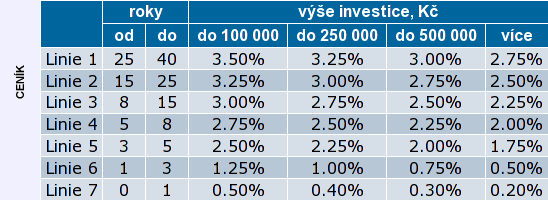
\includegraphics[width=0.8\textwidth]{ri_cost.png}			
			\caption{Poplatky Rentier Invest zdroj: http://www.pioneerinvestments.cz/Rentier/ZakladniInformace.asp}
			\label{ri_cost}
		\end{figure}
\clearpage
\appendix
\section{Poplatky AXA investiční společnost \cite{axa_cite}}
\label{axa}	
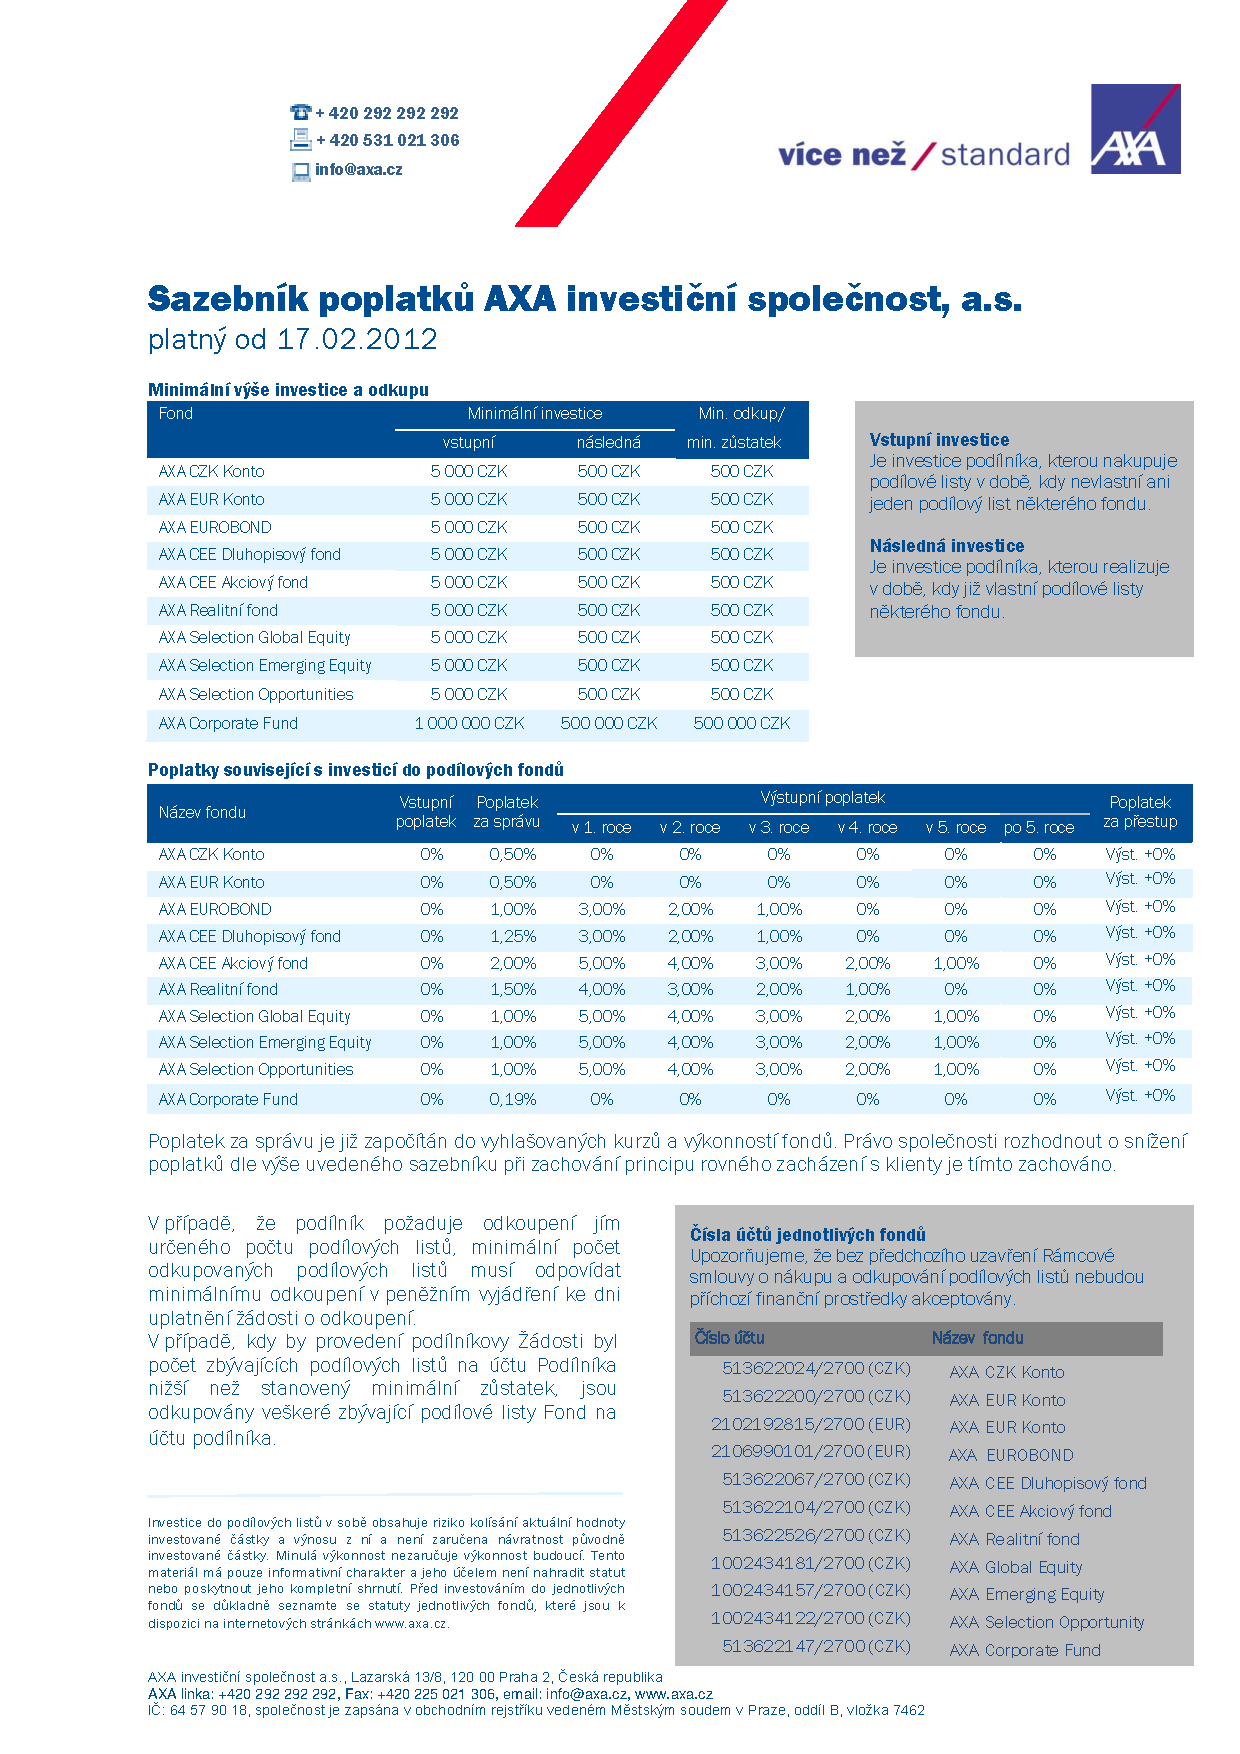
\includegraphics[width=1.0\textwidth]{axa.pdf}
\renewcommand{\bibname}{Seznam použité literatury}
\begin{thebibliography}{9}
\addcontentsline{toc}{chapter}{Seznam použité literatury}
\thispagestyle{plain}

\bibitem{axa_about}
Leták Podílové fondy AXA, [cit. 2012-03-23], Dostupné z WWW:  \url{http://www.axa.cz/getattachment/59ed8936-2745-409d-952b-801213d54a2d/Letak-Podilove-fondy}


\bibitem{axa_cite}
Sazebník poplatků AXA investiční společnost, a.s., [cit. 2012-03-23], Dostupné z WWW:  \url{http://www.axa.cz/getattachment/edb1852e-a78d-4c80-9515-55f0f1db5953/Sazebnik-poplatku}

\bibitem{pio_about}
Pioneer Asset Management, a.s., O společnosti Pioneer Investments [cit. 2012-03-23], Dostupné z WWW:  \url{http://www.pioneerinvestments.cz/Spolecnost.asp}
\end{thebibliography}
\end{document}